
\def \Subject {گزارش پروژه}
\def \Course {درس امنیت سیستم های کامپیوتری}
\def \Author {نیما کمبرانی, فاطمه زهرا بخشنده}
\def \Report {مینی پروژه 1}
\def \StudentNumber {98521423 , 98522157}

\begin{center}
\vspace{.4cm}
{\bf {\huge \Subject}}\\
{\bf \Large \Course}
\vspace{.2cm}
\end{center}
{\bf \Author }  \\
{\bf شماره دانشجویی:\ \StudentNumber}
\hspace{\fill} 
{\Large \Report} \\
\hrule
\vspace{0.8cm}

\clearpage

%\huge{\Subject}\\[1.5 cm]
%\chapterauthor{\Author~ : \StudentNumber}
\par

\section{سوال 1}
\subsection{توضیحات}
در نهان سازی داده ها به روش 
\lr{\b{LSB}}
، ابتدا با گرفتن تصویر و پیام، مخفی سازی شروع می‌شود. پیام مورد نظر در بیت های  
\lr{\b{LSB}}
پیکسل ها ذخیره می شوند. 
در مرحله بعد، برای تشخیص پنهان شدن پیام در تصویر، در پایان پیام یک رشته مشخص افزوده می‌شود. از وجود این رشته در هنگام بازیابی پیام نیز استفاده می‌شود. بدین صورت که با شروع از ابتدا با رسیدن به این رشته مشخص، پایان پیام و همچنین وجود پیام مشخص می‌شود.




\subsection{شکل}
\par

نمونه اجرای کد برای تصویری که در آن پیامی مخفی نشده است در شکل
 \ref{fig:LSBDecode2}
آمده است. همانطور که در شکل پیداست، اگر پیامی در تصویر موجود نباشد، پیام 
\lr{\b{No Hidden Message Found }}
چاپ می‌شود.

\begin{figure}[h!]
    \centering
    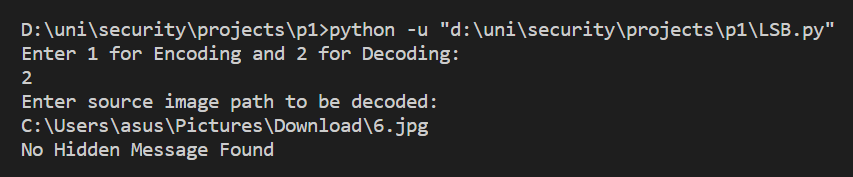
\includegraphics[width=0.5\linewidth]{images/LSB_Decode2.png}
    \caption{خروجی کنسول در هنگام اجرای کد برای شناسایی جمله مخفی شده در تصویر}
    \label{fig:LSBDecode2}
\end{figure}

حال یک پیام را در این شکل نهان سازی می کنیم.

\begin{figure}[h!]
    \centering
    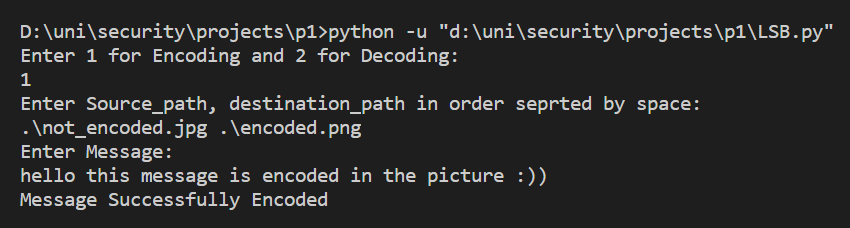
\includegraphics[width=0.5\linewidth]{images/LSB_encode.png}
    \caption{خروجی کنسول در هنگام اجرای کد برای مخفی سازی پیام در تصویر}
    \label{fig:encoded}
\end{figure}

حال می خواهیم پیام نهان سازی شده در این تصویر را تشخیص دهیم.
نمونه اجرای کد برای شناسایی پیام مخفی شده در یک تصویر در شکل
 \ref{fig:LSBDecode}
آمده است.

\begin{figure}[h!]
    \centering
    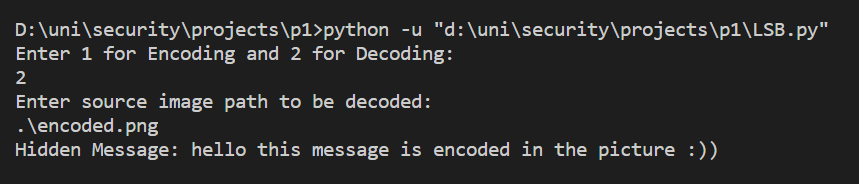
\includegraphics[width=0.5\linewidth]{images/LSB_Decode.png}
    \caption{خروجی کنسول در هنگام اجرای کد برای مخفی سازی پیام در تصویر}
    \label{fig:LSBDecode}
\end{figure}



\subsection{کد سوالات}

کد این سوال با پایتون نوشته شده است. با اجرای کد، ابتدا انتخاب می کنیم که هدف مخفی سازی پیام است یا تشخیص پیام مخفی سازی شده. اگر هدف، تشخیص پیام باشد، آدرس تصویر را از ما خواسته و سپس اگر پیامی در تصویر نهان شده بود، آن را چاپ می کند، و در صورتی که پیامی نبود گزارش می دهد.

اگر هدف مخفی سازی پیام باشد، آدرس تصویر مبدا و مقصد ذخیره سازی را وارد کرده و سپس پیام مورد نظر را جهت نهان سازی وارد می کنیم.

\begin{latin}
\begin{listing}[ht]
    \inputminted{python}{sources/Encode.py}
    \caption{Least Significant Bit steganography Encoder}
    \label{listing:}
\end{listing}
\end{latin}
\begin{latin}
\begin{listing}[ht]
    \inputminted{python}{sources/Decode.py}
    \caption{Least Significant Bit steganography Decoder}
    \label{listing:}
\end{listing}
\end{latin}



\section{سوال 2}

\subsection{توضیحات}
نشانه‌گذاری به افزودن متن یا لوگو بصورت قابل شناسایی یا غیرقابل دیدن به یک تصویر گفته می‌شود. اینکار می‌تواند به منظور حفظ مالکیت یک تصویر و جلوگیری از استفاده از این تصویر بدون اجازه یا با تغییر محتوا صورت پذیرد.
نشانه گذاری هایی مانند افزودن آرم یک شبکه تلویزیونی به تصویر به منظور  جلوگیری از پخش تصویر بدون اجازه یا قرار دادن امضای دیجیتال به همراه فایل تصویر به منظور حفظ صحت عکس از مثال های نشانه گذاری هستند.
در این سوال یک نمونه نشانه گذاری از نوع قابل دیدن (
\lr{visible}
)
و غیرشکننده 
( \lr{non-fragile} ) 
 پیاده‌سازی شده است. در این کد با گرفتن یک لوگو آن را برروی تصویر قرار می‌دهد.













\subsection{نمونه}


\begin{figure}[h!]
    \centering
    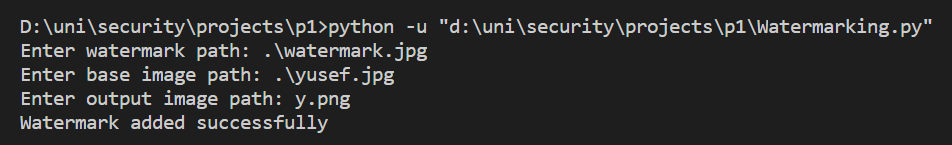
\includegraphics[width=0.5\linewidth]{images/set_watermark.png}
    \caption{خروجی کنسول برای نشان گذاری تصویر}
    \label{fig:watermark}
\end{figure}

\begin{figure}[h!]
    \centering
    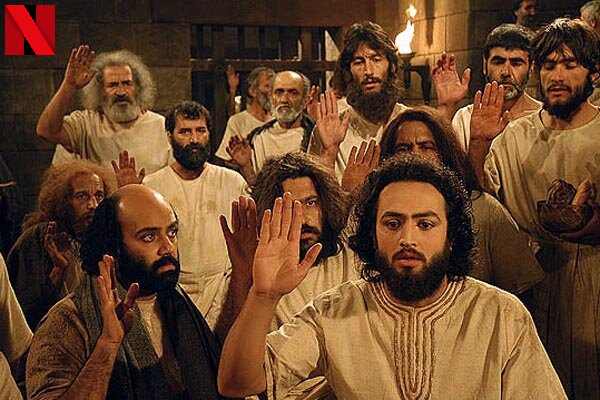
\includegraphics[width=0.5\linewidth]{images/y.png}
    \caption{تصویر به همراه لوگو اضافه شده به آن به عنوان یه نشانه گذاری قابل دیدن و غیر شکننده}
    \label{fig:dynamicprogramming}
\end{figure}

\subsection{کد سوال}
کد سوال با استفاده از زبان پایتون پیاده شده است. در این برنامه با گرفتن آدرس یک تصویر به عنوان لوگو و یک تصویر به‌عنوان تصویر پایه می‌گیرد. سپس با تغییر اندازه لوگو به اندازه 50 در 50 آن را در گوشه تصویر قرار می‌دهد. در نهایت تصویر نهایی در یک فایل جدید ذخیره می‌شود.
\begin{latin}
\begin{listing}[ht]
    \inputminted{python}{sources/Watermarking.py}
    \caption{Adding a logo(visible and non-fragile watermark) to the image implementation}
    \label{code:watermark}
\end{listing}
\end{latin}


